% =====================================================================
%  FIGURAS DEL CAPÍTULO 4 — Diseño de la solución
%  Diagramas vectoriales en TikZ (diseño, no capturas).
%
%  USO EN LA MEMORIA:
%   1. Asegurar en el preámbulo de DocumentoFinalOverleaf.tex:
%        \usepackage{tikz}
%        \usetikzlibrary{positioning, fit, backgrounds, arrows.meta, calc}
%   2. Copiar cada entorno figure[...]...\end{figure} en el lugar marcado
%      con [FIG: ...] del capítulo 4, o usar \input de este fichero.
%   3. Referenciar con \cref{fig:...} (etiquetas indicadas en cada figura).
%
%  Este fichero compila por sí solo para previsualizar (Overleaf):
% =====================================================================
\documentclass[tikz,border=8pt]{standalone}
% --- Si se prefiere previsualizar como documento normal, comentar la
%     línea anterior y descomentar el bloque siguiente: ---
% \documentclass[11pt]{article}
% \usepackage[T1]{fontenc}
% \usepackage[utf8]{inputenc}
% \usepackage[spanish,es-noshorthands]{babel}
% \usepackage{tikz}

\usepackage[T1]{fontenc}
\usepackage[utf8]{inputenc}
\usepackage{pifont}   % \ding{55} (cruz roja); si no se usa, puede omitirse
\usepackage{tikz}
\usetikzlibrary{positioning, fit, backgrounds, arrows.meta, calc}

% ---- Paleta común ----
\definecolor{czona}{RGB}{37,99,235}     % azul zonas/servicios
\definecolor{cweb}{RGB}{16,185,129}     % verde web
\definecolor{cback}{RGB}{139,92,246}    % violeta backend
\definecolor{cdb}{RGB}{6,182,212}       % cian datos
\definecolor{cwarn}{RGB}{220,38,38}     % rojo bloqueo
\definecolor{cok}{RGB}{22,163,74}       % verde ok
\definecolor{cgris}{RGB}{107,114,128}   % gris externo
% Colores de zona (fig. 4 — alta separación cromática)
\definecolor{czoneweb}{RGB}{5,150,105}    % verde esmeralda — web_zone
\definecolor{czoneback}{RGB}{124,58,237}   % violeta — backend_zone
\definecolor{czonedb}{RGB}{217,119,6}     % ámbar — db_zone (no cian: se confunde con verde)

\begin{document}

% =====================================================================
% FIGURA 1 — Pila tecnológica de los microservicios  (§4.1.1, línea 437)
% =====================================================================
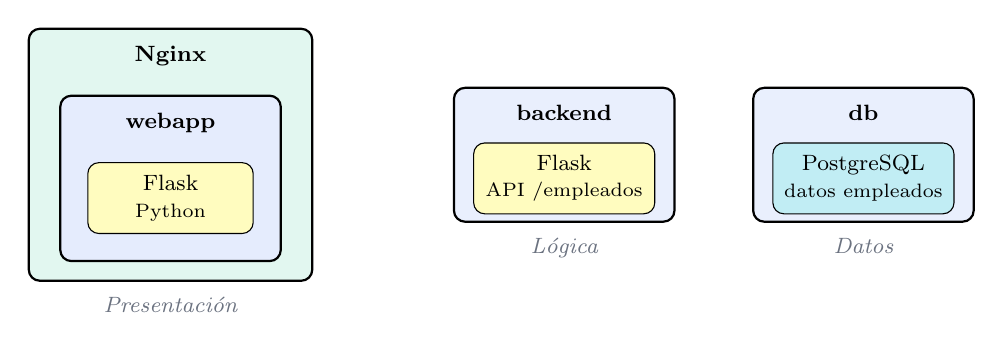
\begin{tikzpicture}[font=\small,
    outerbox/.style={draw, thick, rounded corners, fill=cweb!12},
    innerbox/.style={draw, thick, rounded corners, fill=czona!12},
    tech/.style={draw, rounded corners, fill=yellow!25, align=center, font=\footnotesize},
    box/.style={draw, thick, rounded corners, fill=czona!10},
    layerlabel/.style={font=\footnotesize\itshape, text=cgris}]

  % --- webapp: nginx { webapp { Flask } } ---
  \node[outerbox, minimum width=3.6cm, minimum height=3.2cm] (ng) at (0,0) {};
  \node[anchor=north, font=\footnotesize\bfseries] at ([yshift=-3pt]ng.north) {Nginx};
  \node[innerbox, minimum width=2.8cm, minimum height=2.1cm] (wa) at (0,-0.30) {};
  \node[anchor=north, font=\footnotesize\bfseries] at ([yshift=-3pt]wa.north) {webapp};
  \node[tech, minimum width=2.1cm, minimum height=0.9cm] at (0,-0.55) {Flask\\\scriptsize Python};
  \node[layerlabel, below=2pt of ng] {Presentación};

  % --- backend ---
  \node[box, minimum width=2.8cm, minimum height=1.7cm] (be) at (5.0,0) {};
  \node[anchor=north, font=\footnotesize\bfseries] at ([yshift=-3pt]be.north) {backend};
  \node[tech, minimum width=2.3cm, minimum height=0.9cm] at (5.0,-0.30) {Flask\\\scriptsize API /empleados};
  \node[layerlabel, below=2pt of be] {Lógica};

  % --- db ---
  \node[box, minimum width=2.8cm, minimum height=1.7cm] (db) at (8.8,0) {};
  \node[anchor=north, font=\footnotesize\bfseries] at ([yshift=-3pt]db.north) {db};
  \node[tech, fill=cdb!25, minimum width=2.3cm, minimum height=0.9cm] at (8.8,-0.30) {PostgreSQL\\\scriptsize datos empleados};
  \node[layerlabel, below=2pt of db] {Datos};
\end{tikzpicture}
%
% \begin{figure}[ht]\centering
%   ... (tikzpicture anterior) ...
%   \caption{Pila tecnológica de los tres microservicios del sistema. La
%   aplicación es funcionalmente idéntica en ambos escenarios. Fuente:
%   elaboración propia.}
%   \label{fig:arquitectura-microservicios}
% \end{figure}

\bigskip

% =====================================================================
% FIGURA 2 — Flujo lineal webapp->backend->db  (§4.1.1, línea 449)
% =====================================================================
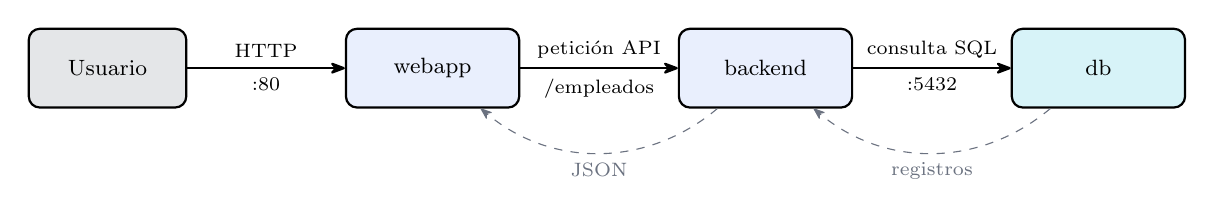
\begin{tikzpicture}[font=\small, >={Stealth[round]}, node distance=2.0cm,
    svc/.style={draw, thick, rounded corners, fill=czona!10, minimum width=2.2cm, minimum height=1.0cm, align=center, font=\footnotesize},
    ext/.style={draw, thick, rounded corners, fill=cgris!18, minimum width=2.0cm, minimum height=1.0cm, align=center, font=\footnotesize}]

  \node[ext] (user) {Usuario};
  \node[svc, right=of user] (wa) {webapp};
  \node[svc, right=of wa] (be) {backend};
  \node[svc, right=of be, fill=cdb!16] (db) {db};

  % flujo de petición (ida)
  \draw[->, thick] (user) -- node[above,font=\scriptsize]{HTTP} node[below,font=\scriptsize]{:80} (wa);
  \draw[->, thick] (wa) -- node[above,font=\scriptsize]{petición API} node[below,font=\scriptsize]{/empleados} (be);
  \draw[->, thick] (be) -- node[above,font=\scriptsize]{consulta SQL} node[below,font=\scriptsize]{:5432} (db);

  % respuesta (vuelta)
  \draw[->, dashed, cgris] (db) to[bend left=40] node[below,font=\scriptsize]{registros} (be);
  \draw[->, dashed, cgris] (be) to[bend left=40] node[below,font=\scriptsize]{JSON} (wa);

  % acceso directo inexistente
  %\draw[->, thick, cwarn, dashed] (wa) to[bend left=45]
  %      node[above,font=\scriptsize, text=cwarn]{\ding{55}~sin acceso directo} (db);
\end{tikzpicture}
%
% NOTA: si \ding no está disponible, sustituir "\ding{55}~" por "X ".
% \caption{Cadena lineal de comunicación entre microservicios: cada
%   servicio habla solo con el contiguo y \texttt{webapp} nunca accede
%   directamente a la base de datos. Fuente: elaboración propia.}
% \label{fig:flujo-microservicios}

\bigskip

% =====================================================================
% FIGURA 3 — Topología red perimetral (Escenario A)  (§4.2.1, línea 467)
% =====================================================================
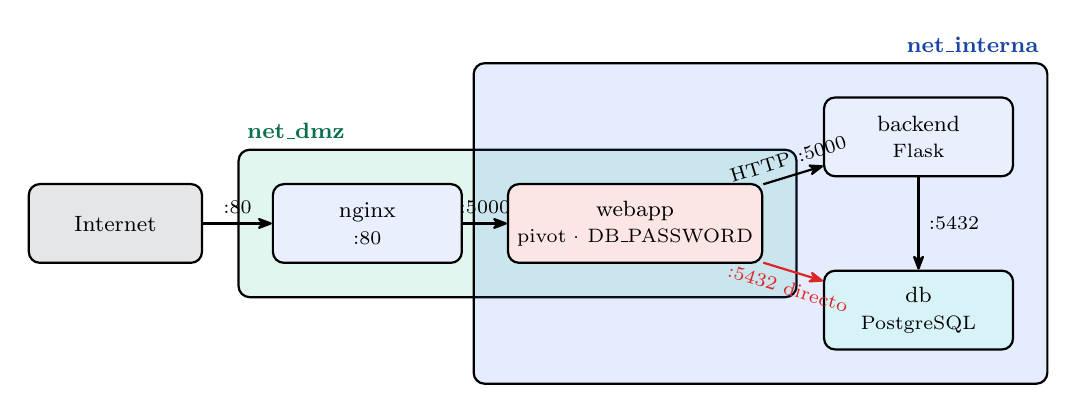
\begin{tikzpicture}[font=\small, >={Stealth[round]},
    svc/.style={draw, thick, rounded corners, fill=czona!10, minimum width=2.4cm, minimum height=1.0cm, align=center, font=\footnotesize},
    ext/.style={draw, thick, rounded corners, fill=cgris!18, minimum width=2.2cm, minimum height=1.0cm, align=center, font=\footnotesize},
    net/.style={draw, thick, rounded corners, inner sep=12pt},
    zlab/.style={font=\footnotesize\bfseries}]

  \node[ext] (net) at (0,0) {Internet};
  \node[svc] (nginx) at (3.2,0) {nginx\\\scriptsize :80};
  \node[svc, fill=cwarn!12] (wa) at (6.6,0) {webapp\\\scriptsize pivot · DB\_PASSWORD};
  \node[svc] (be) at (10.2,1.1) {backend\\\scriptsize Flask};
  \node[svc, fill=cdb!16] (db) at (10.2,-1.1) {db\\\scriptsize PostgreSQL};

  % redes (fondo translúcido)
  \begin{scope}[on background layer]
    \node[net, fill=cweb, fill opacity=0.12, fit=(nginx)(wa)] (dmz) {};
    \node[net, fill=czona, fill opacity=0.12, fit=(wa)(be)(db)] (interna) {};
  \end{scope}
  \node[zlab, text=cweb!60!black, anchor=south west] at (dmz.north west) {net\_dmz};
  \node[zlab, text=czona!70!black, anchor=south east] at (interna.north east) {net\_interna};

  % flujos
  \draw[->, thick] (net) -- node[above,font=\scriptsize]{:80} (nginx);
  \draw[->, thick] (nginx) -- node[above,font=\scriptsize]{:5000} (wa);
  \draw[->, thick] (wa) -- node[above,font=\scriptsize, sloped]{HTTP :5000} (be);
  \draw[->, thick, cwarn] (wa) -- node[below,font=\scriptsize, sloped, text=cwarn]{:5432 directo} (db);
  \draw[->, thick] (be) -- node[right,font=\scriptsize]{:5432} (db);
\end{tikzpicture}
%
% \caption{Topología del Escenario A (perimetral). La segmentación se
%   agota en el perímetro: \texttt{webapp} es multihomed
%   (\texttt{net\_dmz} y \texttt{net\_interna}) y actúa de pivote, con
%   acceso directo y sin control a \texttt{backend} y \texttt{db}.
%   Fuente: elaboración propia.}
% \label{fig:topologia-perimetral}

\bigskip

% =====================================================================
% FIGURA 4 — Topología Zero Trust (Escenario B)  (§4.3.2, línea 503)
% =====================================================================
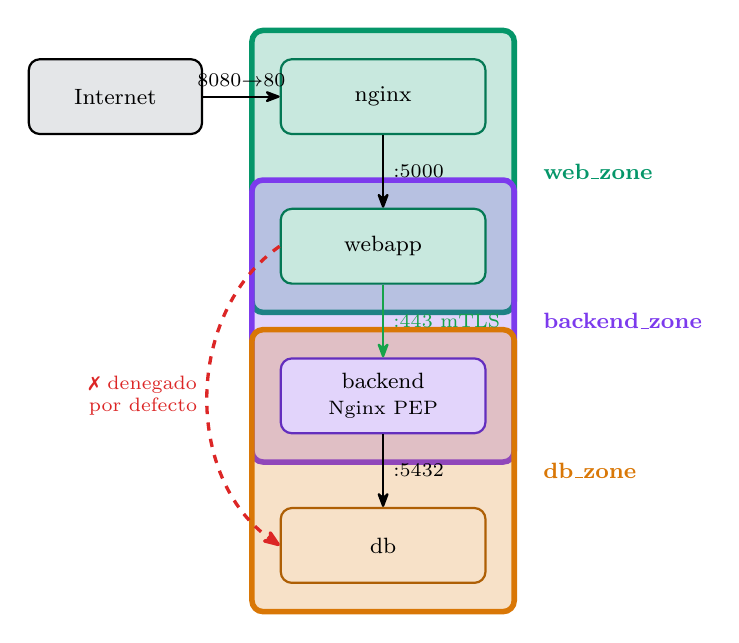
\begin{tikzpicture}[font=\small, >={Stealth[round]},
    svcweb/.style={draw=czoneweb!80!black, thick, rounded corners, fill=czoneweb!22,
      minimum width=2.6cm, minimum height=0.95cm, align=center, font=\footnotesize},
    svcback/.style={draw=czoneback!80!black, thick, rounded corners, fill=czoneback!22,
      minimum width=2.6cm, minimum height=0.95cm, align=center, font=\footnotesize},
    svcdb/.style={draw=czonedb!80!black, thick, rounded corners, fill=czonedb!22,
      minimum width=2.6cm, minimum height=0.95cm, align=center, font=\footnotesize},
    ext/.style={draw, thick, rounded corners, fill=cgris!18, minimum width=2.2cm, minimum height=0.95cm, align=center, font=\footnotesize},
    zone/.style={rounded corners, inner sep=10pt, fill opacity=0.22, text opacity=1, line width=2pt},
    zlab/.style={font=\footnotesize\bfseries}]

  \node[ext] (net) at (-3.4,0) {Internet};
  \node[svcweb] (nginx) at (0,0) {nginx};
  \node[svcweb] (wa)    at (0,-1.9) {webapp};
  \node[svcback] (be)    at (0,-3.8) {backend\\\scriptsize Nginx PEP};
  \node[svcdb] (db) at (0,-5.7) {db};

  % zonas (fondo translúcido; colores bien separados)
  \begin{scope}[on background layer]
    \node[zone, draw=czoneweb, fill=czoneweb, fit=(nginx)(wa)] (wz) {};
    \node[zone, draw=czoneback, fill=czoneback, fit=(wa)(be)]    (bz) {};
    \node[zone, draw=czonedb,   fill=czonedb,   fit=(be)(db)]    (dz) {};
  \end{scope}
  \node[zlab, text=czoneweb,  anchor=west] at ([xshift=6pt]wz.east) {web\_zone};
  \node[zlab, text=czoneback, anchor=west] at ([xshift=6pt]bz.east) {backend\_zone};
  \node[zlab, text=czonedb,   anchor=west] at ([xshift=6pt]dz.east) {db\_zone};

  % flujos permitidos
  \draw[->, thick] (net) -- node[above,font=\scriptsize]{8080$\to$80} (nginx);
  \draw[->, thick] (nginx) -- node[right,font=\scriptsize]{:5000} (wa);
  \draw[->, thick, cok] (wa) -- node[right,font=\scriptsize, text=cok]{:443 mTLS} (be);
  \draw[->, thick] (be) -- node[right,font=\scriptsize]{:5432} (db);

  % flujo denegado webapp -> db
  \draw[->, very thick, cwarn, dashed] (wa.west) to[bend right=55]
        node[left,font=\scriptsize, text=cwarn, align=center]{\ding{55}~denegado\\por defecto} (db.west);
\end{tikzpicture}
%
% \caption{Topología del Escenario B (Zero Trust). Tres zonas con
%   denegación por defecto; \texttt{webapp} y \texttt{backend} son
%   multihomed (zonas solapadas). No existe interfaz común entre
%   \texttt{web\_zone} y \texttt{db\_zone}, por lo que el salto directo
%   \texttt{webapp}$\to$\texttt{db} es imposible. Fuente: elaboración
%   propia.}
% \label{fig:topologia-zerotrust}

\bigskip

% =====================================================================
% FIGURA 5 — Handshake mTLS webapp <-> backend  (§4.3.3, línea 527)
% =====================================================================
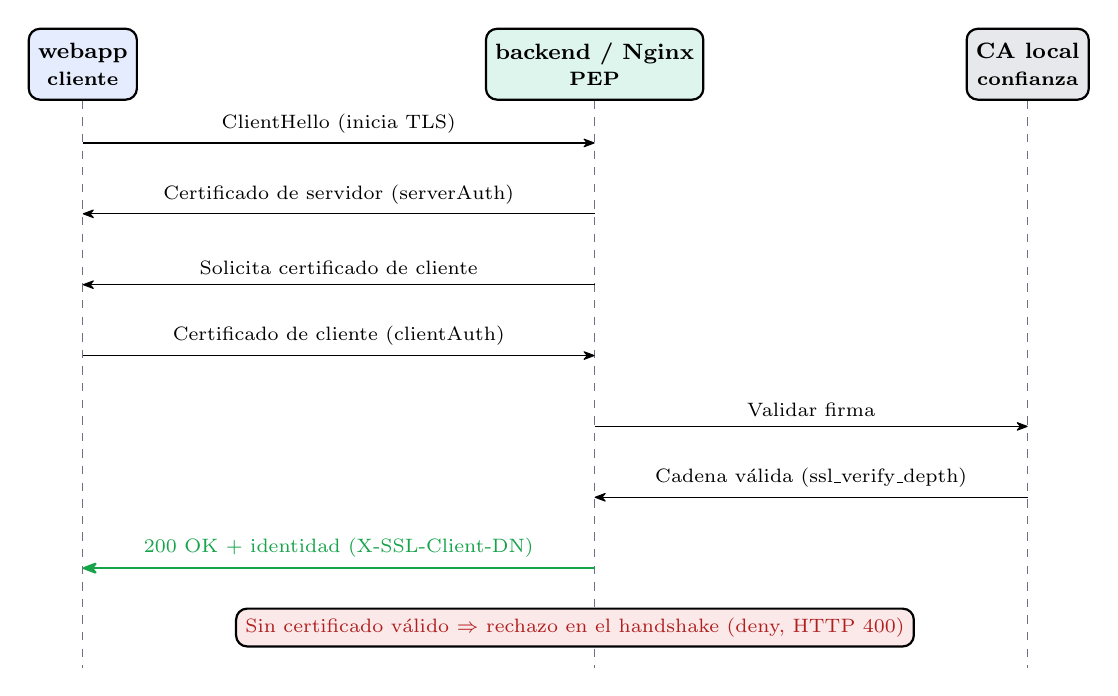
\begin{tikzpicture}[font=\footnotesize, >={Stealth[round]},
    actor/.style={draw, thick, rounded corners, align=center, minimum height=0.9cm, font=\footnotesize\bfseries}]

  \node[actor, fill=czona!12] (W) at (0,0)  {webapp\\\scriptsize cliente};
  \node[actor, fill=cweb!14]  (N) at (6.5,0) {backend / Nginx\\\scriptsize PEP};
  \node[actor, fill=cgris!16] (C) at (12,0) {CA local\\\scriptsize confianza};

  % lifelines
  \foreach \a in {W,N,C} \draw[dashed, cgris] (\a.south) -- ++(0,-7.2);

  \draw[->] (0,-1.0) -- node[above,font=\scriptsize]{ClientHello (inicia TLS)} (6.5,-1.0);
  \draw[<-] (0,-1.9) -- node[above,font=\scriptsize]{Certificado de servidor (serverAuth)} (6.5,-1.9);
  \draw[<-] (0,-2.8) -- node[above,font=\scriptsize]{Solicita certificado de cliente} (6.5,-2.8);
  \draw[->] (0,-3.7) -- node[above,font=\scriptsize]{Certificado de cliente (clientAuth)} (6.5,-3.7);
  \draw[->] (6.5,-4.6) -- node[above,font=\scriptsize]{Validar firma} (12,-4.6);
  \draw[<-] (6.5,-5.5) -- node[above,font=\scriptsize]{Cadena válida (ssl\_verify\_depth)} (12,-5.5);
  \draw[->, cok, thick] (6.5,-6.4) -- node[above,font=\scriptsize, text=cok]{200 OK + identidad (X-SSL-Client-DN)} (0,-6.4);

  % rechazo
  \node[draw, thick, rounded corners, fill=cwarn!10, text=cwarn!80!black, align=center,
        font=\scriptsize, anchor=north] at (6.25,-6.9)
        {Sin certificado válido $\Rightarrow$ rechazo en el handshake (deny, HTTP 400)};
\end{tikzpicture}
%
% \caption{Secuencia de autenticación mutua (mTLS) en el canal
%   \texttt{webapp}$\to$\texttt{backend}. Nginx actúa como punto de
%   aplicación de políticas y exige certificado de cliente firmado por la
%   CA local; sin él, la conexión se rechaza. Fuente: elaboración propia.}
% \label{fig:mtls-handshake}

\bigskip

% =====================================================================
% FIGURA 6 — Ubicación de Wazuh en el modelo Zero Trust (§4.3.4, l. 535)
% =====================================================================
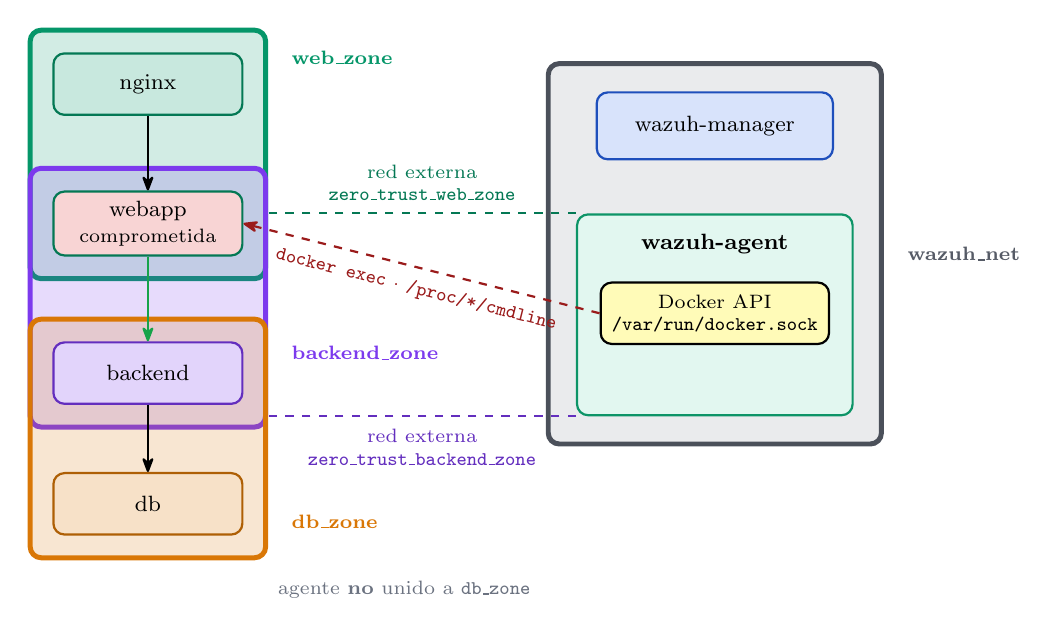
\begin{tikzpicture}[font=\small, >={Stealth[round]},
    svcweb/.style={draw=czoneweb!80!black, thick, rounded corners, fill=czoneweb!22,
      minimum width=2.4cm, minimum height=0.78cm, align=center, font=\footnotesize},
    svcback/.style={draw=czoneback!80!black, thick, rounded corners, fill=czoneback!22,
      minimum width=2.4cm, minimum height=0.78cm, align=center, font=\footnotesize},
    svcdb/.style={draw=czonedb!80!black, thick, rounded corners, fill=czonedb!22,
      minimum width=2.4cm, minimum height=0.78cm, align=center, font=\footnotesize},
    wazmgr/.style={draw=czona!80!black, thick, rounded corners, fill=czona!18,
      minimum width=3.0cm, minimum height=0.85cm, align=center, font=\footnotesize},
    wazagentouter/.style={draw=cweb!80!black, thick, rounded corners, fill=cweb!12,
      minimum width=3.5cm, minimum height=2.55cm},
    dockapi/.style={draw, thick, rounded corners, fill=yellow!28, align=center, font=\scriptsize},
    alertbox/.style={draw=cwarn!70!black, thick, rounded corners, fill=cwarn!12,
      minimum width=3.0cm, minimum height=0.85cm, align=center, font=\footnotesize},
    zonezt/.style={rounded corners, inner sep=8pt, fill opacity=0.18, line width=1.8pt},
    zonewaz/.style={rounded corners, inner sep=10pt, fill opacity=0.14, line width=1.8pt,
      draw=cgris!70!black, fill=cgris},
    compose/.style={font=\footnotesize\bfseries, anchor=west},
    annex/.style={font=\scriptsize, align=center, text=cgris},
    bridge/.style={thick, dashed},
    telem/.style={->, thick}]

  % --- Compose aplicación ZT (izquierda) ---

  \node[svcweb] (nginx) at (0,0.25) {nginx};
  \node[svcweb, fill=cwarn!20] (wa) at (0,-1.52) {webapp\\\scriptsize comprometida};
  \node[svcback] (be) at (0,-3.42) {backend};
  \node[svcdb] (db) at (0,-5.08) {db};

  \begin{scope}[on background layer]
    \node[zonezt, draw=czoneweb, fill=czoneweb, fit=(nginx)(wa)] (wz) {};
    \node[zonezt, draw=czoneback, fill=czoneback, fit=(wa)(be)] (bz) {};
    \node[zonezt, draw=czonedb, fill=czonedb, fit=(be)(db)] (dz) {};
  \end{scope}
  \node[font=\scriptsize\bfseries, text=czoneweb, anchor=west]
        at ([xshift=5pt,yshift=35pt]wz.east) {web\_zone};
  \node[font=\scriptsize\bfseries, text=czoneback, anchor=west]
        at ([xshift=5pt,yshift=-20pt]bz.east) {backend\_zone};
  \node[font=\scriptsize\bfseries, text=czonedb, anchor=west]
        at ([xshift=5pt,yshift=-30pt]dz.east) {db\_zone};

  \draw[telem] (nginx) -- (wa);
  \draw[telem, cok] (wa) -- node[right, font=\scriptsize, text=cok]{} (be);
  \draw[telem] (be) -- node[right, font=\scriptsize]{} (db);

  % --- Compose Wazuh (derecha; 2º stack) ---


  \node[wazmgr] (manager) at (7.2,-0.28) {wazuh-manager};

  % wazuh-agent: contenedor con docker.sock montado en su interior
  \node[wazagentouter] (agentbox) at (7.2,-2.68) {};
  \node[anchor=north, font=\footnotesize\bfseries] at ([yshift=-4pt]agentbox.north) {wazuh-agent};
  % \node[font=\scriptsize, text=cgris] at ([yshift=-14pt]agentbox.north) {multihomed · \texttt{--pid=host}};
  \node[dockapi, minimum width=2.9cm, minimum height=0.78cm] (dock) at (7.2,-2.66)
        {Docker API\\\texttt{/var/run/docker.sock}};
  % \node[annex, anchor=north] at ($(dock.south)+(0,-0.04)$) {
  %   \texttt{process-webapp.sh} (2\,s)\\
  %   \texttt{process-list} (5\,s) · FIM certs
  % };

  \begin{scope}[on background layer]
    \node[zonewaz, fit=(manager)(agentbox)] (wn) {};
  \end{scope}
  \node[font=\scriptsize\bfseries, text=cgris!80!black, anchor=west] at ([xshift=5pt]wn.east) {wazuh\_net};

  % \node[alertbox] (alerts) at (7.2,-4.95) {alerts.json\\\scriptsize reglas 100100--100104};

  % \draw[telem] (agentbox.north) -- node[right, font=\scriptsize]{:1514 / :1515} (manager.south);
  % \draw[telem] (manager) -- node[right, font=\scriptsize]{correlación} (alerts);
  % \node[annex, below=2pt of alerts] {$\to$ KPI G1 (detección)};

  % --- Acoplamiento a redes ZT (external: true) — carriles horizontales separados ---
  \coordinate (webLaneL) at (agentbox.north west);
  \coordinate (webLaneR) at (wz.east |- webLaneL);
  \draw[bridge, czoneweb!80!black] (webLaneL) --
        node[midway, above, font=\scriptsize, align=center, text=czoneweb!80!black, yshift=1pt]
        {red externa\\\texttt{zero\_trust\_web\_zone}}
        (webLaneR);

  \coordinate (backLaneL) at (agentbox.south west);
  \coordinate (backLaneR) at (bz.east |- backLaneL);
  \draw[bridge, czoneback!80!black] (backLaneL) --
        node[midway, below, font=\scriptsize, align=center, text=czoneback!80!black, yshift=-1pt]
        {red externa\\\texttt{zero\_trust\_backend\_zone}}
        (backLaneR);

  \node[font=\scriptsize, text=cgris, align=left, anchor=north west] at ([yshift=-4pt]dz.south east)
        {agente \textbf{no} unido a \texttt{db\_zone}};

  % --- Observación: línea directa docker.sock → webapp ---
  \draw[->, thick, dashed, cwarn!70!black] (dock.west) --
        node[midway, below, font=\scriptsize, align=center, sloped, yshift=-1pt]
        {\texttt{docker exec} · \texttt{/proc/*/cmdline}}
        (wa.east);

  % --- Leyenda de despliegue ---
  % \node[draw, rounded corners, fill=czona!6, inner sep=6pt, font=\scriptsize, align=left,
  %       anchor=north west] at (-0.2,-6.35) {
  %   \textbf{Orden de arranque:} stack ZT $\to$ compose Wazuh $\to$ validación agente.\\
  %   Wazuh \textbf{no altera} la topología medida: se adhiere con \texttt{networks.external}.
  % };
\end{tikzpicture}
%
% \caption{Integración de Wazuh en el Escenario B. El agente se despliega
%   como contenedor con el socket de Docker montado y \texttt{-{}-pid=host};
%   muestrea cada dos segundos los procesos de \texttt{webapp} y envía la
%   telemetría al manager, cuyas reglas generan las alertas que alimentan
%   el indicador de detección. Fuente: elaboración propia.}
% \label{fig:wazuh-zerotrust}

\end{document}
